\documentclass[twoside,12pt,english]{book}
\usepackage{babel}
\usepackage{librebaskerville}
\usepackage[utf8]{inputenc}
\usepackage{xcolor}
\definecolor{marron}{RGB}{60,30,10}
\definecolor{darkblue}{RGB}{0,0,80}
\definecolor{lightblue}{RGB}{80,80,80}
\definecolor{darkgreen}{RGB}{0,80,0}
\definecolor{darkgray}{RGB}{0,80,0}
\definecolor{darkred}{RGB}{80,0,0}
\definecolor{shadecolor}{rgb}{0.97,0.97,0.97}
\usepackage[demo]{graphicx}
\usepackage{wallpaper}
\usepackage{wrapfig,booktabs}

\usepackage{fancyhdr}
\usepackage{lettrine}
\input Acorn.fd
\newcommand*\initfamily{\usefont{U}{Acorn}{xl}{n}}

\usepackage{geometry}
\geometry{
tmargin=5cm, 
bmargin=5cm, 
lmargin=5cm, 
rmargin=3cm,
headheight=1.5cm,
headsep=0.8cm,
footskip=0.5cm}


% \usepackage[full]{textcomp}
\renewcommand{\familydefault}{pplj} 
\usepackage{microtype}

\setlength{\parskip}{1.3ex plus 0.2ex minus 0.2ex}


\usepackage{fourier-orns}

\newcommand{\ornamento}{\vspace{2em}\noindent \textcolor{darkgray}{\hrulefill~ \raisebox{-2.5pt}[10pt][10pt]{\leafright \decofourleft \decothreeleft  \aldineright \decotwo \floweroneleft \decoone   \floweroneright \decotwo \aldineleft\decothreeright \decofourright \leafleft} ~  \hrulefill \\ \vspace{2em}}}
\newcommand{\ornpar}{\noindent \textcolor{darkgray}{ \raisebox{-1.9pt}[10pt][10pt]{\leafright} \hrulefill \raisebox{-1.9pt}[10pt][10pt]{\leafright \decofourleft \decothreeleft  \aldineright \decotwo \floweroneleft \decoone}}}
\newcommand{\ornimpar}{\textcolor{darkgray}{\raisebox{-1.9pt}[10pt][10pt]{\decoone \floweroneright \decotwo \aldineleft \decothreeright \decofourright \leafleft} \hrulefill \raisebox{-1.9pt}[10pt][10pt]{\leafleft}}}

\makeatletter
\def\headrule{{\color{darkgray}\raisebox{-2.1pt}[10pt][10pt]{\leafright} \hrulefill \raisebox{-2.1pt}[10pt][10pt]{~~~\decofourleft \decotwo\decofourright~~~} \hrulefill \raisebox{-2.1pt}[10pt][10pt]{ \leafleft}}}
\makeatother

\fancyhf{}

\renewcommand{\chaptermark}[1]{\markboth{#1}{}}
\renewcommand{\sectionmark}[1]{\markright{#1}}

\newcommand{\estcab}[1]{\itshape\textcolor{marron}{\nouppercase #1}}

\fancyhead[LE]{\estcab{Fran Oldstyle}}
\fancyhead[RE]{\estcab{History of taxonomy}}
% \fancyhead[CE,CO]{\estcab{\decoone}}
\fancyhead[LO]{\estcab{\rightmark}} % malo cuando no hay section ~~~ \thesection
\fancyhead[RO]{\estcab{\leftmark}}

% \fancyhead[RO]{\bf\nouppercase{ \leftmark}}
% \fancyfoot[LE]{\bf \thepage ~~ \leafNE}
% \fancyfoot[RO]{ \leafNE  ~~ \bf \thepage}

\fancyfoot[LO]{
\ornimpar \\ \large \hfill \sffamily\bf \textcolor{darkgray}{\leafNE ~~~ \thepage}
}
\fancyfoot[RE]{\ornpar   \\ \large  \sffamily\bf \textcolor{darkgray}{\thepage ~~~ \reflectbox{\leafNE}}  \hfill}

\newenvironment{Section}[1]
{\section{\vspace{0ex}#1}}
{\vspace{12pt}\centering ------- \decofourleft\decofourright ------- \par}



\usepackage{lipsum}
\setlength{\parindent}{1em} % Sangría española
\pagestyle{fancy}

\renewcommand{\footnoterule}{\vspace{-0.5em}\noindent\textcolor{marron}{\decosix \raisebox{2.9pt}{\line(1,0){100}} \lefthand} \vspace{.5em} }
\usepackage[hang,splitrule]{footmisc}
\addtolength{\footskip}{0.5cm}
\setlength{\footnotemargin}{0.3cm}
\setlength{\footnotesep}{0.4cm} 

\usepackage{chngcntr}
\counterwithout{figure}{chapter}
\counterwithout{table}{chapter}


\begin{document}
\pagecolor{yellow!10}
% \TileWallPaper{300pt}{300pt}{Descargas/fondopapelviejo.jpg}

\chapter{Six kingdoms of life?}
\newpage

\section{Plant\ae}
\lettrine[lines=3]{\initfamily\textcolor{darkgreen}{T}}{he classic} kingdom \emph{Plant\ae} (Haeckel, 1866
include all the multicellular green plants (\emph{Viridiplant\ae} in Latin) as flowering  
plants, conifers, ferns, mosses and green algae. The number of species 
are estimated\footnote{Largely underestimated according to many naturalist.} around 300,000 to 315,000. 
Usually red or brown seaweeds like kelp, fungi and bacteria have
excluded from this group.
This kingdom really exists since Carolus Linn\ae us (1707--1778) who 
divided the natural world into animals, plants and minerals. The kingdom \emph{Animalia}  and \emph{Plant\ae} remained 
in use by modern evolutionary biologists until some years.  

\begin{wrapfigure}{r}{0.26\textwidth}
\centering
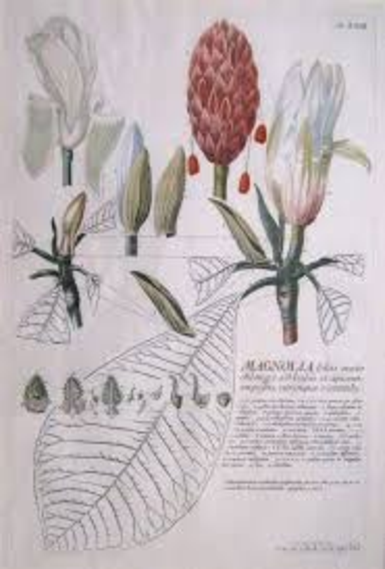
\includegraphics[scale=0.2]{plantae.pdf}
\caption{\footnotesize \emph{Vallaris pergularia} from \emph{Icones plantarum}, vol. II., (Hooker, 1837).}
\label{fig1}
\end{wrapfigure}
But now, both kingkoms are considered only two brachs of the unicelular kingdom \emph{Protist} 
or \emph{Protozoa}\footnote{Although by tradition,  inconsistently the status of kingdom 
is maintained \emph{Animalia}  and \emph{Plant\ae}.}.  
\lipsum[2]

\lipsum[3]

\ornamento

\section{Fungi}

\lettrine[lines=3]{\initfamily\textcolor{darkgreen}{L}}{arlegy}, organism like \emph{Candida albicans} has
 been considered different of \emph{Protozoa} and related with green plants. However, today there 
 are evidences that animals and true fungi are indeed closer to each other than to any other group 
 in the eukaryote tree, far from the alveolates and other eukaryotic lineages.  

\begin{wraptable}{r}{7 cm}
\vspace{-.5cm}
\centering
\footnotesize
\caption{\label{wraptab}Estimated fungal species.}
\begin{tabular}{lr}\\\toprule  
Authors & Species \\\midrule
Bisby and Ainsworth (1943) & $10^5$ \\  
Martin (1951) &  $2.5\times10^5$  \\
Hawksworth (1991) & $1.5\times10^6$ \\ 
O’Brien \emph{et al.} (2005) & $>3.5\times10^6$ \\  \bottomrule
\end{tabular}
\end{wraptable} 


\lipsum[4-6]

\end{document}